% Este archivo es parte de la memoria del proyecto fin de carrera
% de Manuel López Urbina. Protegida bajo la licencia GFDL.
% Para más información, la licencia completa viene incluida en el
% fichero fdl-1.3.tex

% Copyright (C) 2017 Manuel López Urbina

\chapter{Introducción}
\label{chap:introducción}

\emph{Lo mejor que podemos hacer por otro\\ no es sólo compartir con él nuestras riquezas,\\ sino mostrarle las suyas\\ Benjamin Disraeli}\\


\section{Introducción y antecedentes}
\label{sec:introduccion_y_antecedentes}

La robótica es una rama de la ingeniería, la cual se ocupa del diseño, construcción, operación y uso de robots\footnote{Robot: Máquina automática programable capaz de realizar determinadas operaciones de manera autónoma y sustituir a los seres humanos en algunas tareas, en especial las pesadas, repetitivas o peligrosas; puede estar dotada de sensores, que le permiten adaptarse a nuevas situaciones.}, así como sistemas informáticos para su control, retroalimentación sensorial y procesamiento de información. Entre las diversas disciplinas aplicadas a la robótica podemos encontrar: la mecánica, la electrónica, la informática, la inteligencia artificial, la ingeniería de control y la física, entre otras muchas. En conclusión, podemos considerar la robótica como una ciencia multidisciplinar.\\

En la actualidad, los robots comerciales e industriales son ampliamente utilizados y cada día realizan tareas de forma más exacta o más barata que los humanos. También se les utiliza en trabajos demasiado sucios, peligrosos o tediosos. Los robots son muy utilizados en plantas de fabricación, montaje y embalaje, en transporte, en exploraciones en la Tierra y en el espacio, cirugía, armamento, investigación en laboratorios y en la producción en masa de bienes industriales o de consumo. Otras aplicaciones incluyen la limpieza de residuos tóxicos, minería, búsqueda y rescate de personas y localización de minas terrestres. En definitiva, la robótica está presente en prácticamente cualquier ámbito que podamos imaginar en la actualidad.\\

Por otra parte, ninguno de los sistemas robóticos actuales podrían ser funcionales sin un software adecuado para su manejo y control, en ocasiones siendo éste tremendamente complejo y específico para garantizar una correcta sincronización entre los diferentes elementos hardware y software implicados con la finalidad de garantizar un correcto funcionamiento del conjunto robótico.\\

Por estas razones, cada vez son más las escuelas que hacen uso de la robótica para que los estudiantes se interesen en la tecnología ya que puden encontrar un entorno divertido donde aprender, y que ofrece multitud de ventajas: 

\begin{enumerate}
\item {Los niños lo encuentran divertido}
Hay varios concursos orientados a distintos grupos de edad que pueden canalizar la competencia de una manera positiva. Por ejemplo, se le puede pedir a los niños que construyan un robot y luego hacer competiciones.\\
\item{Es una manera eficaz de enseñarles programación a los estudiantes}
La programación puede ser muy abstracta. Al tener que controlar un robot físico y ver lo que sale mal, los estudiantes aprenden lo que los robots pueden y no pueden hacer. También aprenden la necesidad de dar instrucciones precisas.\\
\item{ Desarrolla habilidades útiles}
Capacidad de resolución de problemas, trabajo en equipo, capacidad de análisis, y un largo etcétera.
\end{enumerate}

AÑADIR MAS VENTAJAS


De lo anterior se extrae la necesidad de elaborar un sistema que, además de acercar la robótica a los estudiantes, permita compartir las creaciones con otros usuarios en internet. Todos hemos visto alguna vez vídeos en las redes sociales donde los usuarios nos muestran sus dispositivos en funcionamiento donde, en ocasiones, nos gustaría poder tomar control sobre ellos o visualizar su manejo en tiempo real.\\

Por tanto el sistema resultante debe cubrir dos necesidades principales, la primera, dotar al usuario de las herramientas necesarias para permitir la configuración de una interfaz de control de sus dispositivos sin necesidad de amplios conocimientos de programación, y la segunda, cubrir la necesidad paralela en la que los usuarios, orgullosos de sus creaciones, dispongan de una manera de compartir sus robots con el resto del mundo de una manera más dinámica. Es decir, en la que otros usuarios, a modo de espectadores, puedan visualizar el control de los dispositivos por parte de su creador, como si de una sesión de vídeo en streaming se tratara. También se dotará de la posibilidad de permitir el control por otros usuarios externos. En la actualidad no existe ningún medio eficaz donde hacer una difusión de la robótica de una manera similar.\\

Dada la problemática actual presentada, junto con que la programación web y la robótica son temas que causan en mi un especial interés, hicieron que me lanzara a la elaboración de este proyecto que unifica ambos campos anteriormente citados.\\

Así surgió \emph{RobotUI} y con él un nuevo concepto llamado \textit{RobotSharing}.\\

\begin{figure}[H]
  \begin{center}
    
\includegraphics[scale=0.3]{imagenes/logotipo.png}
  \end{center}
  \label{fig:logo}
 \caption{Logo RobotUI \protect\footnotemark.}
\end{figure}

\footnotetext{Logotipo RobotUI.}

\emph{RobotUI} (nombre del sistema resultante) será una combinación de un elemento software (aplicación web) y hardware (vehículo de pruebas y demostración) surgido como muestra de la solución obtenida a los citados problemas.\\


El elemento hardware de este proyecto se compone de un vehículo controlado vía WiFi el cual responde a una serie de señales \emph{comandos} a los que responde realizando determinadas acciones. La interfaz web se configurará de tal manera que permita el control del susodicho vehículo.\\

\begin{figure}[H]
  \begin{center}
    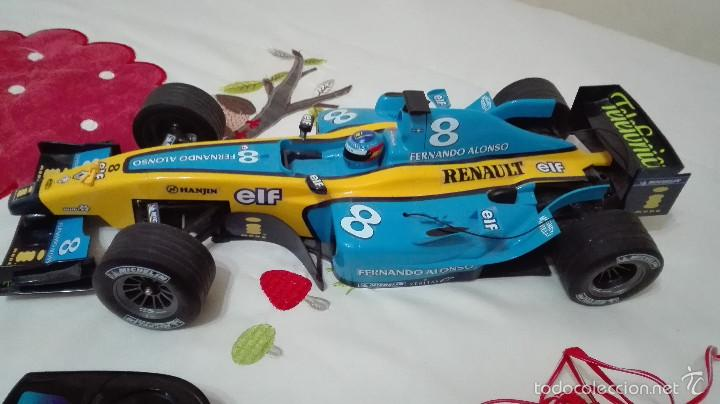
\includegraphics[scale=0.3]{imagenes/f1.jpg}
  \end{center}
  \label{fig:logo}
 \caption{Vehículo utilizado \protect\footnotemark.}
\end{figure}

\footnotetext{Vehículo utilizado.}



\section{Objetivos}
\label{sec:objetivos}

Como hemos visto, se requiere de multitud de conocimientos a la hora de afrontar un proyecto robótico con ciertas garantías. Este proyecto trata, al menos, de reducir, o facilitar, el área relacionada con la informática, más concretamente con la programación. En la que multitud de personas ven en la programación un impedimento a la hora de comenzar a desarrollar sus ideas.
Por otro lado, existe la imperiosa necesidad de que la comunidad quiera mostrar sus creaciones al resto del mundo, compartir experiencias, problemas opiniones, etc, de una forma directa y no
mediante la grabación de vídeos del funcionamiento de los proyectos robóticos en cuestión, ya que no disponen de una herramienta adecuada para ello. En definitiva, existe la necesidad de que otros
usuarios puedan participar de manera más activa, ya sea visualizando el control por su creador o permitir que otros usuarios tomen el control de esos proyectos en tiempo real.
Por tanto este proyecto busca facilitar la árdua labor de programación de los proyectos robóticos junto con la posibilidad de compartir las creaciones realizadas con otros usuarios.\\

El sistema a desarrollar, por tanto, dispondrá de dos modos de funcionamiento, el primero de ellos proporciona las herramientas para la configuración de una interfaz a gusto del usuario, en la cual, una vez configurada, el usuario podrá controlar a su antojo el dispositivo. En el segundo modo de funcionamiento, la aplicación permitirá que otros usuarios puedan visitar la interfaz anteriormente configurada y actuar como espectadores en el control del robot por el usuario propietario del mismo. En definitiva, se proporcionará un sistema de control y difusión en uno solo.\\

\section{Acerca de este documento}

El documento se ha sido elaborado en un lenguaje claro y sencillo para permitir que un estudiante universitario de Ingeniería Informática pueda comprender los contenidos sin apenas dificultad añadida.\\

Este documento se organiza en los siguientes capítulos:\\

\begin{itemize}

\item En el capítulo \ref{chap:introducción}, Introducción, se comentan las razones que han motivado la creación de este proyecto, así como el propósito del mismo.

\item En el capítulo \ref{chap:conceptos-básicos}, Conceptos básicos, se incluyen definiciones de aquellos conceptos considerados de interés para la correcta comprensión del contenido de la presente memoria.

\item En el capítulo \ref{chap:herramientas}, Herramientas utilizadas, se realiza una descripción de las diferentes elementos hardware y software empleados durante el desarrollo del proyecto y necesarios para la utilización del mismo.

\item En el capítulo \ref{chap:organización-temporal}, Organización temporal, se recoge todo lo que concierne a la distribución y duración de cada una de las tareas llevadas a cabo durante el desarrollo del proyecto que el presente documento describe.

\item En el capítulo \ref{chap:dispositivos-hardware}, Configuración y montaje de los dispositivos hardware, se explica el proceso seguido para la correcta integración de los dispositivos hardware empleados describiendo la interconexión entre ellos así como su configuración. 

\item En el capítulo \ref{chap:desarrollo-software}, Desarrollo software, se realiza un análisis sobre la metodología empleada para el desarrollo software, describiendo los modelos de ciclo de vida utilizados, la descripción de los requisitos funcionales junto con el diagrama de casos de uso.

\item En el capítulo \ref{chap:reconocimiento}, Software de reconocimiento, se hace una descripción explicando los diferentes aspectos y elementos de cada uno de los prototipos desarrollados junto con los problemas encontrados y soluciones adoptadas.

\item En el capítulo \ref{chap:software-de-control}, Software de control, se describe cómo se ha llevado a cabo la comunicación ordenador-vehículo a nivel software.

\item En el capítulo \ref{chap:interfaz-gráfica}, Interfaz gráfica, se recogen aquellos aspectos técnicos de interés referentes a la elaboración de la interfaz gráfica.

\item En el capítulo \ref{chap:manual-usuario}, Guía de usuario, se describen los diferentes aspectos necesarios para la correcta utilización del conjunto software y hardware de los que se compone el presente proyecto.

\item En el capítulo \ref{chap:conclusiones}, Conclusiones, se hace mención de las conclusiones obtenidas tras la realización del proyecto además de las posibles mejoras aplicables.

\item En el capítulo Anexos \ref{chap:anexos}, aparecen los manuales de instalación del software que ha sido necesario para la realización del proyecto.

\end{itemize}
